\section{Einphasen-Stromrichteröltrafo 16.7 Hz}
Der \SI[]{16.7}[]{\Hz} Transformator ist ein Summiertransformator und addiert die
Teilspannungen der Umrichter auf die Bahnspannung 2 AC
\SI[]{110}[]{\kV}. Der Transformator ist ölgefüllt, selbstkühlend und für die Aussenaufstellung ausgelegt.

\subsection{Allgemeine Merkmale}

\begin{table}[htb]
    \centering
    \begin{NiceTabular}{|l|c|}[]
        \CodeBefore
        \columncolor{lightergray}{1}
        \Body
        \hline
         Aufstellung & Freiluftaufstellung\\
         \hline
         Verschmutzung & Verschmutzungsgrad III (stark) \\
         \hline
         Aufstellungshöhe & < 1000 m üNN\\
         \hline
         Umgebungstemperatur &  -30°C bis 40°C\\
         \hline
         Klimabedingungen & Normal\\ 
         \hline
                 \Block{3-1}{Dokumentationen} &  \tabitem Technische Zeichnungen und CAD\\
                         &\tabitem Montageplan, Wartungsplan, Dokumentationen\\
                         &\tabitem Prüfprotokoll der zu erfüllenden Prüfungen\\
            \hline
    \end{NiceTabular}
\end{table}

\textbf{Normen:}

\subsubsection*{Schaltbild}
\begin{figure}[htb]
\centering
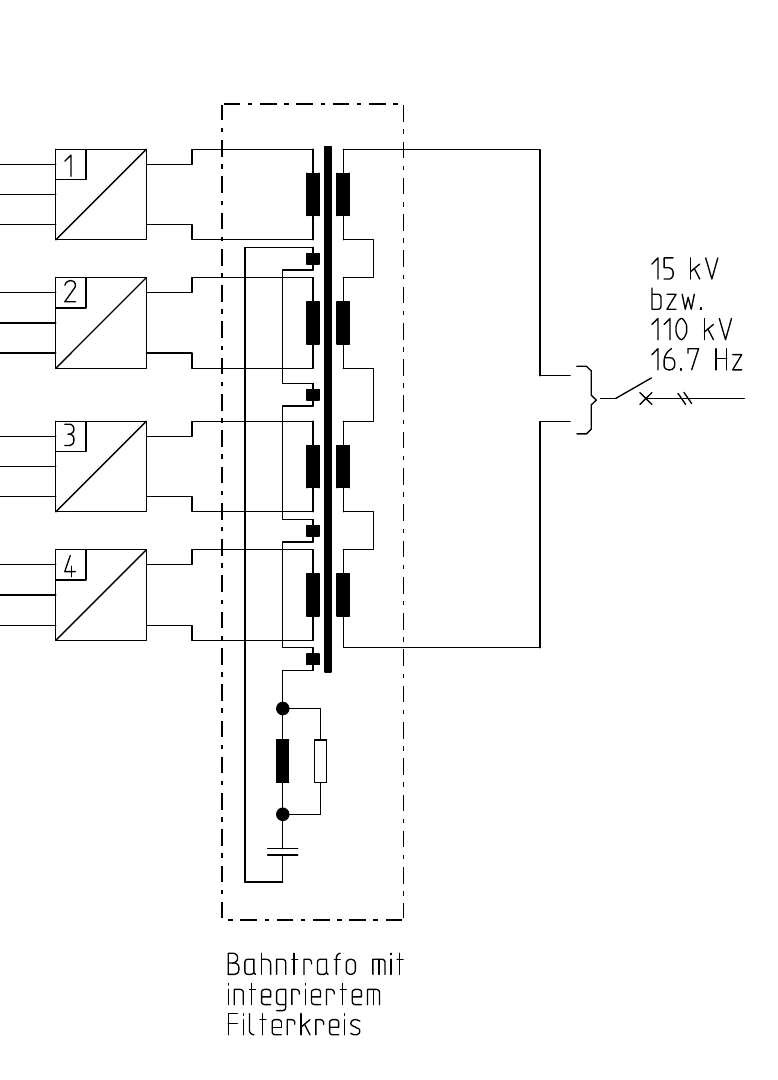
\includegraphics[width=\textwidth/3,frame]{Bilder/stromrichtertrafo.png}
\end{figure}

\subsection{Bemessungsdaten:}
\begin{table}[htb]
    \centering
    \begin{NiceTabular}{|l|p{2cm}|p{2cm}|}[hvlines]
        \CodeBefore
        \columncolor{lightergray}{1}
        \Body
       \Block{2-1}{Schaltgruppe} & OS & US \\ 
                                & | &   i0i0i0  \\
         Nennleistung ohne Leistung der Filterwicklung & \Block{1-2}{$\SI{20}{\unit{\mega\volt\ampere}}$}\\
         Leistung US Wicklung & \Block{1-2}{$4\cdot\SI{5.125}{\mega\VA}$}\\
         Nennfrequenz nach DIN EN 50163/A1 \cite{DeutschesInstitutfurNormungene.V..200802} & \Block{1-2}{$\SI{16.7}{\Hz}-6\%+4\%$}\\
         Nennspannung der OS-Wicklung  & \Block{1-2}{$\SI{110}{\kilo\V}$}\\
         Nennspannung einer US Wicklung bei \SI[]{110}[]{\kV} & \Block{1-2}{$4\cdot\SI{3535}{\kV}$}\\
         Nennstrom US-Wicklung bei Nennspannung & \Block{1-2}{$\SI{1414}{\A}$}\\
        Filterwicklung (HW) Nennleistung & \Block{1-2}{$\SI{4.8}{\mega\VA}$}\\
        Filterwicklung (HW) Nennspannung & \Block{1-2}{$\SI{6}{\kilo\V}$}\\
    \end{NiceTabular}
\end{table}

\subsubsection{Kurzschlussspannung, Impedanzen}
\tabitem 112 MVA; 110kV, beide US-Wicklungen kurzgeschlossen \ang{75}C
\begin{table}[htb]
    \centering
    \begin{NiceTabular}{|l|c|}[hvlines]
        \CodeBefore
        \columncolor{lightergray}{1}
        \Body
        OS-HW& $15\pm \SI[]{5}[]{\percent}(\SI[]{14.225}{\percent}...\SI[]{15.75}[]{\percent})$\\   
        US-HW& $\SI[]{9.4}[]{\percent}$\\
        US-HW& $\SI[]{5.6}[]{\percent}$\\
    \end{NiceTabular}
\end{table}

\subsubsection*{Verluste}
\begin{table}[htb]
    \centering
    \begin{NiceTabular}{|l|c|c|}[hvlines]
        \CodeBefore
        \columncolor{lightergray}{1}
        \Body
       &Grudnschwingung&Umrichterbetrieb(Zusatzverluste)\\
       Leerlaufverluste bei Nennspannung&tbd. \unit{\kW}& < \SI[]{1}[]{\percent} von der Grudnschwingung\\
    Kurzschlussverluste bei \ang{75}C&tbd. \unit{\kW}&< \SI[]{1}[]{\percent} von der Grudnschwingung\\
    \end{NiceTabular}
\end{table}

\subsubsection*{Isolation}
Die Blitzstoß- so wie die angelegte Stehwechselspannungsprüfung (ACSD)  muss als Stückprüung nach DIN EN 60076-3\cite*{DINEN600763VDE0532763:201903.} für alle Wicklungen des Transformators durchgeführt werden.
\begin{table}[htb]
    \centering
    \begin{NiceTabular}{|l|c|c|c|}[]
        \CodeBefore
        \columncolor{lightergray}{1}
        \Body
        &OS&US&FW\\
        \hline
       max. Betriebsspannung Leiter gegen Erde  &  \SI{123}{\kilo\V} & \SI{17.5}{\kilo\V} & \SI{7.2}{\kilo\V}\\
       \hline
       Nennstehwechselspannung gegen Erde & $U_1=$\SI{185}{\kilo\volt}; $U_2=$\SI{230}{\kilo\volt} & \SI{38}{\kilo\V} & \SI{20}{\kilo\V}\\
        \hline  
     \Block{2-1}{Nennstehblitzspannung} &$U_1=$\SI{550}{\kilo\volt}&$U_1=$\SI{95}{\kilo\volt}&$U_1=$\SI{60}{\kilo\volt}\\
        & $U_2=$\SI{450}{\kilo\volt}& $U_2=$\SI{75}{\kilo\volt}&$U_2=$\SI{40}{\kilo\volt}\\
        \bottomrule
    \end{NiceTabular}
\end{table}
\subsubsection*{Kapazitive Kopplung}
Eine kapazitive Übertragung von Blitzüberspannungen von der OS-Wicklung auf die US-Wicklung ist zu vermeiden. Bisherige Transformatoren in Bahnkupplungen hatten zu diesem Zweck Schirmwicklungen. 
 
\subsubsection*{Anschlüsse}

\begin{table}[htb]
    \centering
    \begin{NiceTabular}{l|cccc}[]
        \CodeBefore
        \columncolor{lightergray}{1}
        \Body
        &&OS&US&FW\\
        \hline
            Anzahl der Durchführungen & Klemme&2&4x2&2\\
        \hline
        Art der Durchführung & Klemme & Porzellan & Porzellan & Porzellan\\
        \hline
    \end{NiceTabular}
\end{table}
Anschlusskabel Filter in einem Klemmkasten; 1 Kabel á  \SI{50}{\mm\squared} je  Anschluss  Filterwicklung

\subsubsection*{Stromwandler}
